\section{Overview of MTConnect}

MTConnect is a data and information exchange standard that is based on a \gls{data dictionary} of terms describing information associated with manufacturing operations.  The standard also defines a series of \glspl{semantic data model} that provide a clear and unambiguous representation of how that information relates to a manufacturing operation.  The MTConnect Standard has been designed to enhance the data acquisition capabilities from equipment in manufacturing facilities, to expand the use of data driven decision making in manufacturing operations, and to enable software applications and manufacturing equipment to move toward a plug-and-play environment to reduce the cost of integration of manufacturing software systems.

The MTConnect standard supports two primary communications methods – \gls{requestresponse} and \gls{publishsubscribe} type of communications.  The \gls{requestresponse} communications structure is used throughout this document to describe the functionality provided by MTConnect.  See \sect{Streaming Data} for details describing the functionality of the \gls{publishsubscribe} communications structure available from an \gls{agent}. 

Although the MTConnect Standard has been defined to specifically meet the requirements of the manufacturing industry, it can also be readily applied to other application areas as well.

The MTConnect Standard is an open, royalty free standard – meaning that it is available for anyone to download, implement, and utilize in software systems at no cost to the implementer.

The \glspl{semantic data model} defined in the MTConnect Standard provide the information required to fully characterize data with both a clear and unambiguous meaning and a mechanism to directly relate that data to the manufacturing operation where the data originated.  Without a \gls{semantic data model}, client software applications must apply an additional layer of logic to raw data to convey this same level of meaning and relationship to manufacturing operations.  The approach provided in the MTConnect Standard for modeling and organizing data allows software applications to easily interpret data from a wide variety of data sources which reduces the complexity and effort to develop applications.

The data and information from a broad range of manufacturing equipment and systems are addressed by the MTConnect Standard.  Where the \gls{data dictionary} and \glspl{semantic data model} are insufficient to define some information within an implementation, an implementer may extend the \gls{data dictionary} and \glspl{semantic data model} to address their specific requirements.  See \sect{Extensibility} for guidelines related to extensibility of the MTConnect Standard.

To assist in implementation, the MTConnect Standard is built upon the most prevalent standards in the manufacturing and software industries.  This maximizes the number of software tools available for implementation and provides the highest level of interoperability with other standards, software applications, and equipment used throughout manufacturing operations.  

Current MTConnect implementations are based on HTTP as a transport protocol and \gls{xml} as a language for encoding each of the \glspl{semantic data model} into electronic documents.  All software examples provided in the various MTConnect Standard documents are based on these two core technologies.  

The base functionality defined in the MTConnect Standard is the \gls{data dictionary} describing manufacturing information and the \glspl{semantic data model}.  The transport protocol and the programming language used to represent or transfer the information provided by the \glspl{semantic data model} are not restricted in the standard to HTTP and \gls{xml}.  Therefore, other protocols and programming languages may be used to represent the semantic models and/or transport the information provided by these data models between an \gls{agent} (server) and a client software application as may be required by a specific implementation.

\begin{note}
Note: The term "document" is used with different meanings in the MTConnect Standard:
\begin{itemize}

\item Meaning 1:  The MTConnect Standard itself is comprised of multiple documents each addressing different aspects of the Standard.  Each document is referred to as a Part of the Standard.

\item Meaning 2:  In an MTConnect implementation, the electronic documents that are published from a data source and stored by an \gls{agent}.     

\item Meaning 3:  In an MTConnect implementation, the electronic documents generated by an \gls{agent} for transmission to a client software application. 
\end{itemize}

The following will be used throughout the MTConnect Standard to distinguish between these different meanings for the term "document":

\begin{itemize}

\item MTConnect Document(s) or Document(s) shall be used to refer to printed or electronic document(s) that represent a Part(s) of the MTConnect Standard.  

\item All reference to electronic documents that are received from a data source and stored in an \gls{agent} shall be referred to as "\gls{document}(s)" and are typically provided with a prefix identifier; e.g. \gls{asset document}.

\item All references to electronic documents generated by an \gls{agent} and sent to a client software application shall be referred to as a "\gls{response document}".  
\end{itemize}

When used with no additional descriptor, the form "document" shall be used to refer to any printed or electronic document.
\end{note}

Manufacturing software systems implemented utilizing MTConnect can be represented by a very simple structure as shown in \fig{basic-mtconnect-implementation-structure}.

\begin{figure}[ht]
  \centering
  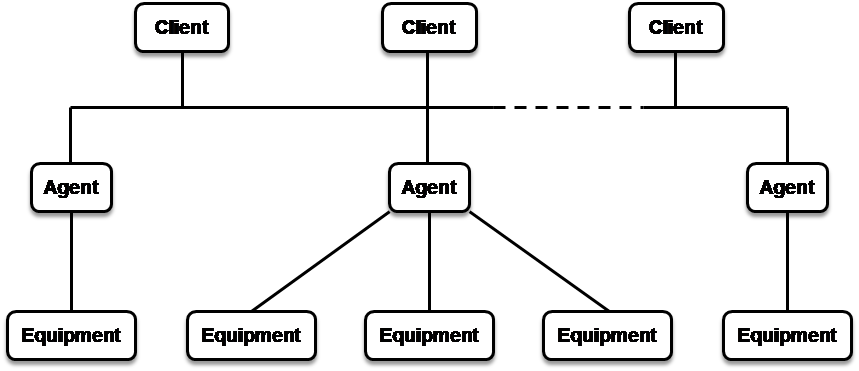
\includegraphics[width=1.0\textwidth]{figures/basic-mtconnect-implementation-structure.png}
  \caption{Basic MTConnect Implementation Structure}
  \label{fig:basic-mtconnect-implementation-structure}
\end{figure}

\FloatBarrier

The three basic modules that comprise a software system implemented using MTConnect are:

\ulheading{Equipment}:  Any data source.  In the MTConnect Standard, equipment is defined as any tangible property that is used to equip the operations of a manufacturing facility.  Examples of equipment are machine tools, ovens, sensor units, workstations, software applications, and bar feeders.

\ulheading{\gls{agent}}:  Software that collects data published from one or more piece(s) of equipment, organizes that data in a structured manner, and responds to requests for data from client software systems by providing a structured response in the form of a \gls{response document} that is constructed using the \glspl{semantic data model} defined in the Standard. 

\begin{note}
Note:	The \gls{agent} may be fully integrated into the piece of equipment or the \gls{agent} may be independent of the piece of equipment.  Implementation of an \gls{agent} is the responsibility of the supplier of the piece of equipment and/or the implementer of the \gls{agent}.
\end{note}
    
\ulheading{Client Software Application}:  Software that requests data from \glspl{agent} and processes that data in support of manufacturing operations. 

Based on \fig{basic-mtconnect-implementation-structure}, it is important to understand that the MTConnect Standard only addresses the following functionality and behavior of an \gls{agent}:

\begin{itemize}

\item the method used by a client software application to request information from an \gls{agent}.

\item the response that an \gls{agent} provides to a client software application.

\item a \gls{data dictionary} used to provide consistency in understanding the meaning of data reported by a data source.

\item the description of the \glspl{semantic data model} used to structure \glspl{response document} provided by an \gls{agent} to a client software application.

\end{itemize}

These functions are the primary building blocks that define the \gls{base functional structure} of the MTConnect Standard.

There are a wide variety of data sources (equipment) and data consumption systems (client software systems) used in manufacturing operations.  There are also many different uses for the data associated with a manufacturing operation.  No single approach to implementing a data communication system can address all data exchange and data management functions typically required in the data driven manufacturing environment.  MTConnect has been uniquely designed to address this diversity of data types and data usages by providing different \glspl{semantic data model} for different data application requirements:

\ulheading{Data Collection}: The most common use of data in manufacturing is the collection of data associated with the production of products and the operation of equipment that produces those products.  The MTConnect Standard provides comprehensive \glspl{semantic data model} that represent data collected from manufacturing operations.  These \glspl{semantic data model} are detailed in \citetitle{MTCPart2} and \citetitle{MTCPart3} of the MTConnect Standard.

\ulheading{Inter-operations Between Pieces of Equipment}:  The MTConnect Standard provides an \gls{interaction model} that structures the information required to allow multiple pieces of equipment to coordinate actions required to implement manufacturing activities.  This \gls{interaction model} is an implementation of a \gls{requestresponse}  messaging structure.  This \gls{interaction model} is called \gls{interfaces component} which is detailed in \citetitle{MTCPart5} of the MTConnect Standard.

\ulheading{Shared Data}:  Certain information used in a manufacturing operation is commonly shared amongst multiple pieces of equipment and/or software applications.  This information is not typically "owned" by any one manufacturing resource.  The MTConnect Standard represents this information through a series of \glspl{semantic data model} – each describing different types of information used in the manufacturing environment.  Each type of information is called an \gls{mtconnect asset}. \glspl{mtconnect asset} are detailed in \citetitle{MTCPart40}, and its sub-Parts, of the MTConnect Standard.

\section{Purpose of This Document}

This document, \citetitle{MTCPart1} of the \gls{mtconnect}  Standard, addresses two major topics relating to the MTConnect Standard.  The first sections of the document define the organization of the documents used to describe the MTConnect Standard; including the terms and terminology used throughout the Standard.  The balance of the document defines the following:

\begin{itemize}
\item Operational concepts describing how an \gls{agent} should organize and structure data that has been collected from a data source.

\item Definition and structure of the \glspl{response document} supplied by an \gls{agent}.

\item The protocol used by a client software application to communicate with an \gls{agent}.
\end{itemize}

\section{Terminology and Conventions} \label{sec:Terminology and Conventions} 

\printglossary

%\printacronyms  

\printbibliography[title=MTConnect References,keyword=MTC]

%Use
%\nocite{*}
%to list all the references; used or unused

\printbibliography[title=Other References,notkeyword=MTC]

\nolinenumbers
\glsaddallunused
\nolinenumbers

\linenumbers